% !TeX spellcheck = it_IT
\section{Cosa sono i Bitcoin?}

Bitcoin è una valuta elettronica creata nel 2008 da Satoshi Nakamoto, uno pseudonimo dietro al quale non si sa ancora con la precisione chi si nasconde.
Con il termine Bitcoin viene denotata sia la rete che consente il possesso e il trasferimento di denaro, sia la moneta. Per convenzione, Bitcoin si riferisce alla tecnologia della rete, mentre \textit{bitcoin} alla valuta stessa.\cite{wiki:bitcoin}

Come ogni valuta, i bitcoin possono essere trasferiti tramite gli utenti, grazie ad un protocollo che viene rispettato all'interno della rete Internet, il quale può essere eseguito su differenti dispositivi, in modo tale da permettere la fruibilità del servizio anche attraverso gli smartphones.
 
I bitcoins possono essere comprati, venduti e scambiati con altre valute, tramite degli organismi specializzati nel cambio di monete virtuali. In un certo senso, Bitcoin è la forma perfetta di denaro per Internet, dal momento che è estremamente veloce, sicuro e senza limiti.

A differenza delle altre valute, i bitcoin sono esclusivamente virtuali, dietro di essi non esistono monete fisiche. Tali bitcoin vengono coinvolti in transazioni da mittente a ricevente, i quali possiedono delle chiavi crittografiche pubbliche e private che servono per trasmettere e sbloccare la spesa dei bitcoin ricevuti.
Infatti, senza la chiave privata, chi riceve i bitcoin non può spenderli in nessun modo. Tali chiavi vengono conservate all'interno di un \textit{wallet}, letteralmente un "portafoglio". Ogni wallet è caratterizzato da un indirizzo Bitcoin il quale è univoco e ha la funzione di fare riferimento ad uno dei partecipanti alla transazione. In questo modo, quando viene effettuato uno scambio di bitcoin, vengono visualizzati solamente gli indirizzi dei wallet. Questa caratteristica permette quindi di rendere anonime le transazioni, dato che agli indirizzi non è connesso in nessun modo il nome o il cognome dell'individuo o dell'associazione che interviene nello scambio.

La rete Bitcoin, oltre ad essere completamente virtuale, è priva di un'unità centralizzata, infatti essa è costituita da un sistema distribuito peer-to-peer.\\
I bitcoin vengono creati tramite un processo, detto \textit{mining}, che permette a chiunque di mettersi in competizione per trovare una soluzione ad un problema matematico. Ogni persona che partecipa alla rete bitcoin, potrebbe operare come un \textit{miner}, ovvero colui che cerca di risolvere il problema matematico per generare bitcoin, usando le capacità del proprio computer messo a disposizione della computazione.\cite{antonopoulos2014mastering}\\

Quando viene effettuato uno scambio di bitcoin tra due o più wallet, viene creata una \textit{transazione}. Ogni transazione viene conservata in una struttura dati chiamata \textbf{blocco}, il quale a sua volta va a costituire la \textbf{Blockchain}.

\subsection{Bitcoin: Panoramica}

Nella \textit{figura\ref{fig:overview}}, si può notare che il sistema bitcoin comprende: utenti con wallet che contengono chiavi, transazioni che sono propagate attraverso la rete, e miner che forniscono (attraverso una computazione competitiva) il consenso alla blockchain, la quale è il libro mastro di tutte le transazioni. 

In questo paragrafo si andrà a tracciare il percorso di una singola transazione quando viene propagata attraverso la rete, e le interazioni tra ogni componente del sistema, ad alto livello.

\begin{figure}[h]
	\centering
	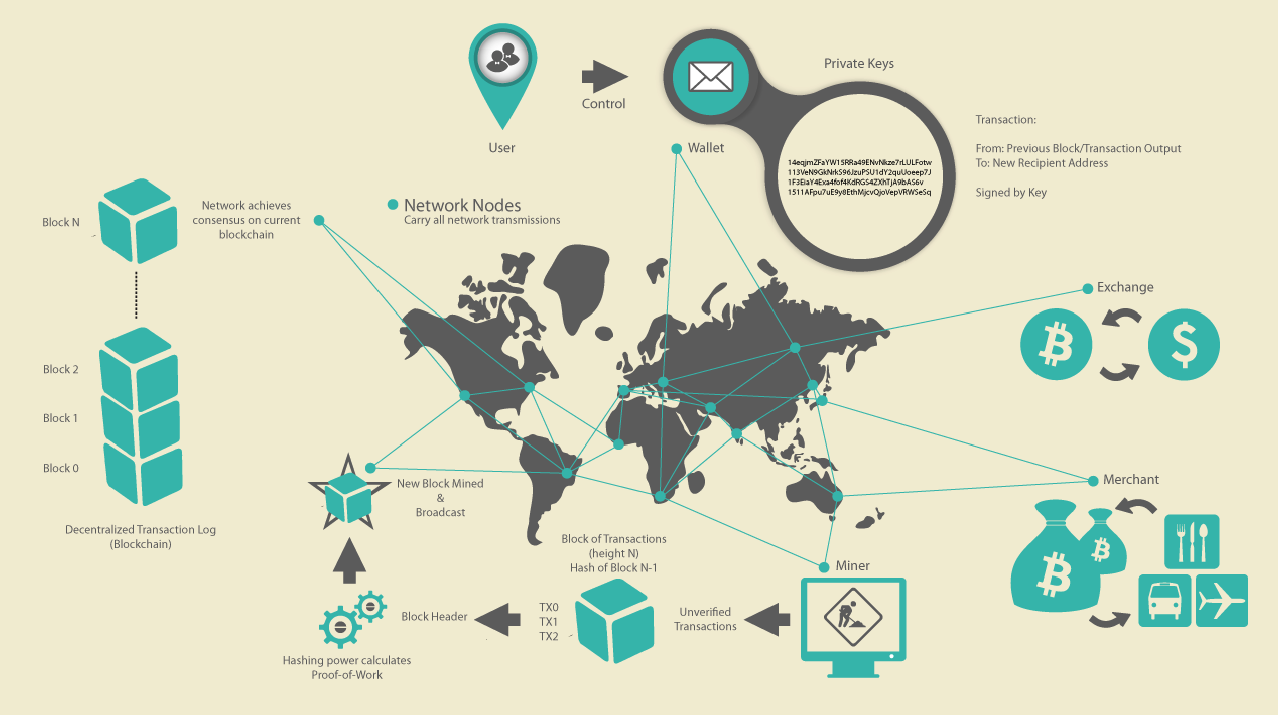
\includegraphics[width= \linewidth]{figure/overview}
	\caption{\textit{Bitcoin overview} \label{fig:overview}}
\end{figure}

Si prendano in considerazione per esempio, due utenti Bitcoin: Alice e Bob. Alice vorrebbe effettuare la sua transazione, comprando una tazza di caffè al bar di Bob (Bob's Cafe). Il bar di Bob, di recente ha iniziato ad accettare pagamenti in bitcoin, aggiungendo alla cassa un punto di pagamento Bitcoin. I prezzi del bar sono elencati in dollari, ma alla cassa, i clienti hanno l'opzione di pagare sia in dollari che in bitcoin.

Alice fa il suo ordine di una tazza di caffè e Bob inserisce la transazione nel registratore di cassa. Il punto di scambio di bitcoin, converte il prezzo totale dai dollari ai bitcoin secondo il tasso di mercato corrente, e mostra il prezzo nelle due valute, insieme ad un QR code contenente la \textit{payment request} (richiesta di pagamento) per tale transazione (\textit{figura \ref{fig:qrcode}}).
\begin{figure}[h]
	\centering
	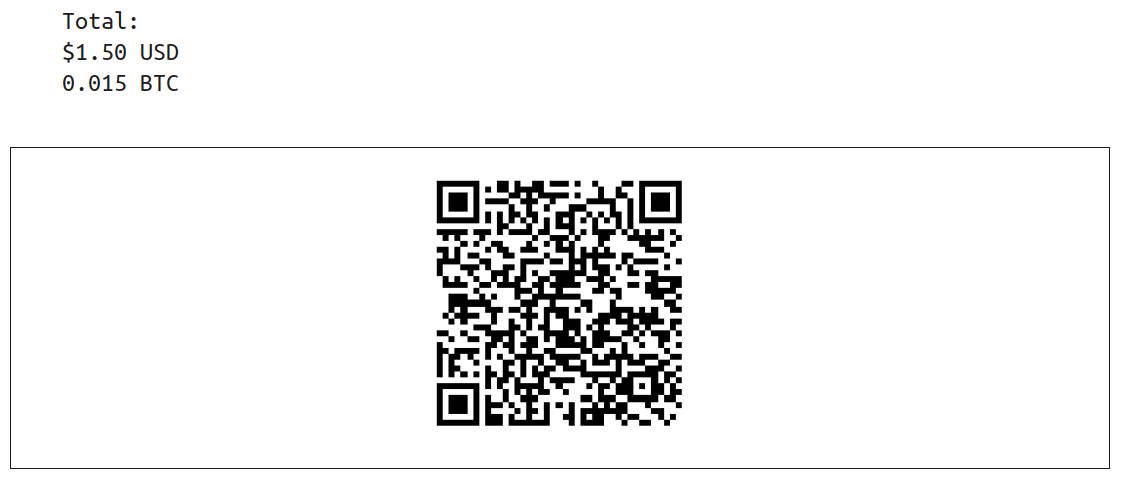
\includegraphics[width= 0.8 \linewidth]{figure/qrcode}
	\caption{\textit{Payment request QR code} \label{fig:qrcode}}
\end{figure}

Se tale QR code viene scansionato, esso racchiude il seguente URL:
\begin{lstlisting}
	bitcoin:1GdK9UzpHBzqzX2A9JFP3Di4weBwqgmoQA?
	amount=0.015&
	label=Bob%27s%20Cafe&
	message=Purchase%20at%20Bob%27s%20Cafe
\end{lstlisting}

Attraverso di esso si possono ottenere informazioni come: l'indirizzo bitcoin, l'ammontare del pagamento, un'etichetta per l'indirizzo del destinatario e una descrizione del pagamento.

A differenza di un QR code che contiene semplicemente l'indirizzo bitcoin del destinatario, un \textit{payment request} è un QR-encoded URL che contiene un indirizzo di destinazione, il pagamento, e una descrizione generica come "Bob's Cafe". Questo permette all'applicazione del wallet di raccogliere le  informazioni usate per effettuare il pagamento, al fine di mostrarle successivamente quando richieste dal proprietario del wallet. Se Bob scansiona il QR code con un'applicazione per un wallet bitcoin, oltre a ottenere il denaro, vedrà i dettagli inseriti da Alice.

Quindi, Bob dice: "Sono un dollaro e 50, oppure 15 millibitcoin"

Alice usa il suo smartphone per cansionare il codice e visualizzarlo sul display. Esso le mostra il pagamento di 0.015 BTC al Bob's Cafe e seleziona \textit{Invia} per autorizzare il pagamento. In pochi secondi (all'incirca lo stesso tempo che ci mette una comune carta di credito), Bob potrà vedere la transazione sul registratore di cassa, conclusa.\cite{antonopoulos2014mastering}

\section{Cos'è la Blockchain?}
La Blockchain, letteralmente \textit{catena di blocchi}, è una base di dati distribuita, che permette la memorizzazione delle transazioni raggruppate in blocchi connessi tra loro, ognuno con il suo successivo. Ogni blocco è una struttura dati che contiene un numero variabile di transazioni, inserite dal \textit{miner} che ha minato il blocco, fino ad un tetto massimo di 1MB per singolo blocco.\\

L'idea di base della Blockchain, deriva dal concetto di \textbf{libro mastro}, il registro della contabilità in cui sono riuniti tutti i conti che compongono un dato sistema contabile. In questo caso il sistema contabile sarebbe la rete Bitcoin, mentre la Blockchain sarebbe il libro mastro che contiene tutti i conti, ovvero le transazioni. \\

L'antico libro mastro, veniva utilizzato come fonte ufficiale per la memorizzazione degli scambi e dei passaggi di proprietà. Infatti, quando veniva fatta una compravendita tra mittente e ricevente, veniva controllato sul libro mastro se il ricevente non avesse speso precedentemente il denaro, e se il mittente non avesse già venduto la merce usata nello scambio.

Infine, se fosse andato tutto a buon fine, veniva registrata la transazione sul libro mastro, in modo da essere consultabile e pubblica per le successive transazioni.

Un principio importante di questo meccanismo è la fiducia, la quale tutti ripongono nel libro mastro: ognuno si fida del gestore della memorizzazione delle transazioni, al punto che, chi compra e chi vende, può effettuare scambi anche senza fidarsi reciprocamente. Quindi, il libro mastro è una garanzia, sia per il mittente che per il ricevente dello scambio. Inoltre, le banche possono perciò controllare gli scambi che vengono fatti e il denaro posseduto da ogni partecipante alle transazioni.

La Blockchain, come già sottolineato, è una struttura dati composta da diverse unità di base, dette blocchi. Infatti, blockchain significa letteralmente \textit{catena di blocchi}.

Quindi, tali blocchi vengono "incatenati", ovvero collegati tra loro tramite un protocollo ben definito nella struttura del sistema bitcoin. 

Ogni blocco all'interno della blockchain, è identificato da un codice hash, generato applicando l'algoritmo di crittografia SHA256 all'header del blocco. Un singolo blocco è collegato al suo predecessore, conosciuto come "blocco genitore", attraverso il campo \textit{previous block hash} all'interno del proprio header. In altre parole, ogni blocco contiene l'hash del proprio blocco genitore all'interno dell'header. Infine, la sequenza dei vari hash genera una catena che collega tutti i blocchi all'indietro, fino al blocco numero zero.\cite{antonopoulos2014mastering}

\subsection{Mining}

Le monete bitcoin sono "coniate" durante la creazione di ciascun blocco ad un tasso fisso. Ogni blocco, generato all'incirca ogni 10 minuti, contiene nuovi bitcoin, creati da zero.
Il \textit{mining} inoltre serve per proteggere il sistema bitcoin contro transazioni fraudolente o transazioni che cercano di spendere gli stessi bitcoin più di una volta, problema conosciuto con il nome di \textit{double-spend} (doppia-spesa).

I miner validano le transazioni e le registrano sul \textit{ledger} globale, ovvero la Blockchain, creando un nuovo blocco e inserendo le transazioni al suo interno, per poi aggiungere il blocco alla chain (=catena). Perciò, i miner raccolgono un certo numero di transazioni e cercano di inserirle all'interno di un nuovo blocco creato appositamente. Tutte le transazioni che poi risultano alla fine all'interno di tale blocco, sono considerate \textit{confirmed} (=confermate), ovvero una sorta di etichetta che permette al ricevente di tali bitcoin di spenderli successivamente.

Lo scopo dei miner è quello di guadagnare bitcoin, e possono ottenerli in due modi: 
\begin{itemize}
	\item quando un nuovo blocco viene aggiunto alla Blockchain, si ottiene un premio in bitcoin
	\item per ogni transazione vengono pagate le \textit{fees} (=tasse) al miner
\end{itemize}

Al fine di ottenere il premio, i miner devono trovare la soluzione ad un problema matematico molto difficile basato su un algoritmo di crittografia. La soluzione a tale problema, chiamata \textbf{proof of work}, è inclusa all'interno del nuovo blocco, e serve come prova che il miner ha impiegato un notevole sforzo di elaborazione. La competizione tra i miner per trovare la proof of work per guadagnare bitcoin è alla base della sicurezza del sistema Bitcoin.

Il processo della generazione di nuove monete è chiamato \textbf{mining} perchè la ricompensa è progettata in modo da simulare rendimenti decrescenti, esattamente come l'estrazione di metallo prezioso.
La fornitura di valuta bitcoin è creata attraverso il mining, analogamente alla procedura con cui una banca centrale crea moneta stampando banconote. 

L'ammontare del premio del mining a Gennaio 2009 era di 50 bitcoin per blocco e a Novembre 2012 già si era dimezzato fino ad ottenere 25 bitcoin. Attualmente il guadagno del premio del mining risulta 12.5 bitcoin per blocco.
Seguendo questo processo, il premio per il mining di un blocco, decrescerà esponenzialmente fino all'anno 2140, quando tutti i bitcoin (20.9999998 milioni) saranno emessi. All'incirca dopo il 2140 non saranno più prodotti nuovi bitcoin e il miner andrà a guadagnare solamente tramite le tasse applicate per ogni transazione.

I miners guadagnano bitcoin per ogni transazione tramite le tasse. Esse vengono calcolate come eccesso di bitcoin tra le transazioni di input e quelle di output. Infatti, il miner che riesce a creare il nuovo blocco "tiene il resto" di ogni transazione inclusa in quel blocco. \\ Dopo il 2140, tutti i bitcoin potranno essere guadagnati tramite tasse.

La parola "mining", ovvero minare, potrebbe avere un significato ingannevole poichè sembrerebbe indicare l'estrazione di metallo prezioso, e quindi focalizza l'attenzione sul premio che viene ottenuto dal minatore.\\
Sebbene il mining sia incentivato dal suo guadagno, il suo obiettivo principale non è il premio in denaro o la creazione di nuove monete.\\ 
Mining è il processo principale per la decentralizzazione del sistema, nel quale le transazioni sono validate e chiare. Rappresenta una sicurezza per il sistema e permette lo sviluppo di una rete basata sul consenso, senza l'intervento di un'autorità centrale.\cite{antonopoulos2014mastering}

Quando un blocco viene minato, ovvero viene aggiunto alla blockchain, viene etichettato con un timestamp, che rappresenta l'istante in cui viene ricevuto dal nodo bitcoin che ha la copia della blockchain.

\subsection{Consenso Decentralizzato}

La Blockchain non essendo creata da un'autorità centrale, è assemblata indipendentemente da ogni nodo all'interno della rete. Perciò, ogni nodo della rete, agendo sulle informazioni che vengono trasmesse attraverso delle connessioni di rete non sicure, può arrivare alla stessa conclusione e assemblare una copia della stessa blockchain, come ogni altro nodo.

La principale invenzione di Satoshi Nakamoto è il meccanismo decentralizzato del \textit{consenso emergente}. "Emergente" perchè il consenso generale non è raggiunto esplicitamente -- non esiste un'elezione o un momento prefissato quando il consenso viene espresso -- è un risultato dell'interazione asincrona di migliaia di nodi indipendenti tra loro, i quali basati sulle stesse regole.

Tutte le proprietà dei bitcoin, inclusa la moneta, le transazioni, i pagamenti, il modello di sicurezza, i quali non dipendono da un'autorità centrale, derivano da questa invenzione.\\
Il consenso decentralizzato dei Bitcoin viene fuori dall'interazione di quattro processi che si verificano indipendentemente sui nodi attraverso la rete. Tali processi sono:
\begin{itemize}
	\item la verifica indipendente di ogni transazione, basata su una lista globale di criteri
	\item  l'aggregazione indipendente di tali transazioni all'interno di un nuovo blocco appena minato
	\item la verifica indipendente del nuovo blocco da parte di ogni nodo, e l'unione di tale blocco all'interno della chain
	\item la selezione indipendente, da parte di ogni nodo, della chain con la computazione che maggiormente raccoglie più transazioni e che è stata dimostrata correttamente tramite una \textit{proof of work}
\end{itemize}
\cite{antonopoulos2014mastering}

\subsection{Blockchain Forks}

Dal momento che la Blockchain è una struttura dati decentralizzata, copie differenti non sono sempre consistenti. Infatti, i blocchi possono arrivare a nodi diversi in tempi diversi, creando differenti rami all'interno della stessa blockchain.

Sebbene un blocco abbia solo un genitore, esso può avere temporaneamente un diverso numero di figli. Ogni figlio si riferisce allo stesso blocco genitore e contiene lo stesso hash del genitore nel campo  \textit{previous block hash}. Questa temporanea molteplicità di figli può causare una \textit{fork} (letteralmente \textit{biforcazione}), ovvero una situazione in cui blocchi differenti vengono creati quasi simultaneamente da diversi miners.

Per risolvere il problema della biforcazione, ogni nodo Bitcoin seleziona sempre e cerca di estendere la catena di blocchi che soddisfa il sistema \textit{proof-of-work}.

Le fork avvengono come risultato di inconsistenze temporanee tra versioni della blockchain,
che vengono risolte con eventuali riconvergenze, ovvero i nuovi blocchi vengono aggiunti alla catena principale della biforcazione.

Nelle figure seguenti, si può capire un esempio di una fork della blockchain. Sebbene nelle figure si nota la rete globale, in realtà la topologia della rete bitcoin non è organizzata geograficamente, piuttosto forma una rete di nodi interconnessi, che potrebbero essere geograficamente molto lontani. Nella vera rete bitcoin, la \textit{distanza} tra i nodi è misurata in \textbf{hop} da nodo a nodo, non sulla loro distanza fisica. Un singolo hop è una porzione di percorso tra la sorgente e la destinazione. 

Per scopi illustrativi, blocchi differenti sono mostrati con colori diversi, che si diffondono attraverso la rete e le connessioni attraversate vengono colorate con colori diversi.
Nel primo diagramma (\textit{figura \ref{fig:fork1}}), la rete appare con una singola prospettiva unificata della blockchain, con il blocco blu come estremità della catena principale.
\begin{figure}[h]
	\centering
	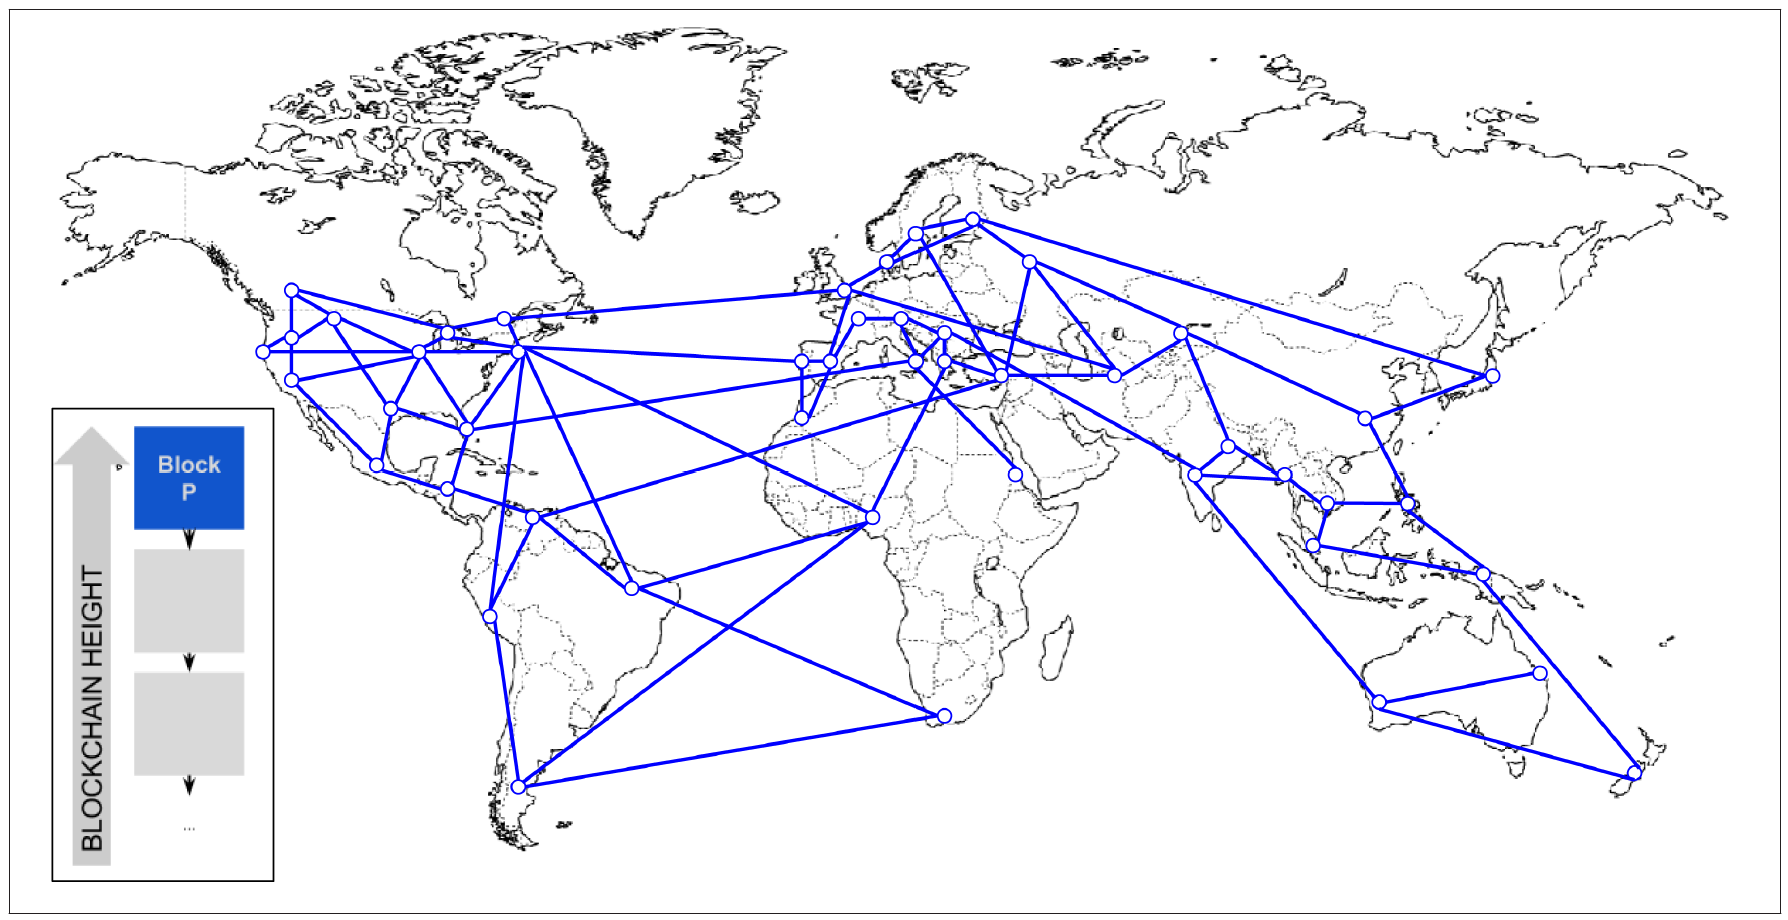
\includegraphics[width=0.85 \linewidth]{figure/fork1}
	\caption{\textit{Visualizzazione di un evento fork--prima della fork} \label{fig:fork1}}
\end{figure}

Un evento \textit{fork} avviene quando ci sono due diversi blocchi che sono candidati ad essere aggiunti contemporaneamente alla Blockchain. Ciò può accadere quando due diversi miner risolvono la proof of work con uno scarto di tempo molto piccolo tra entrambi. Di conseguenza, tali miner immediatamente rivelano la loro soluzione in modo broadcast, e il nuovo blocco creato viene trasmesso tempestivamente ai loro vicini, che propagano i blocchi nuovi attraverso la rete. 

Ogni nodo che riceve un blocco valido, lo incorpora all'interno della propria versione della blockchain, allungandola di un blocco. Se tale nodo si rende conto di aver ricevuto un ulteriore blocco che soddisfa le condizioni, lo aggiunge creando una catena secondaria alternativa al blocco aggiunto appena prima.

In \textit{figura \ref{fig:fork2}} si possono notare due miner che hanno minato due diversi blocchi quasi simultaneamente.\\
Entrambi i blocchi sono figli del blocco blu, ed hanno lo scopo di estendere la chain aggiungendosi sopra al blocco blu. Nella figura, un blocco è rappresentato in rosso e l'altro in verde.
\begin{figure}[htbp]
	\centering
	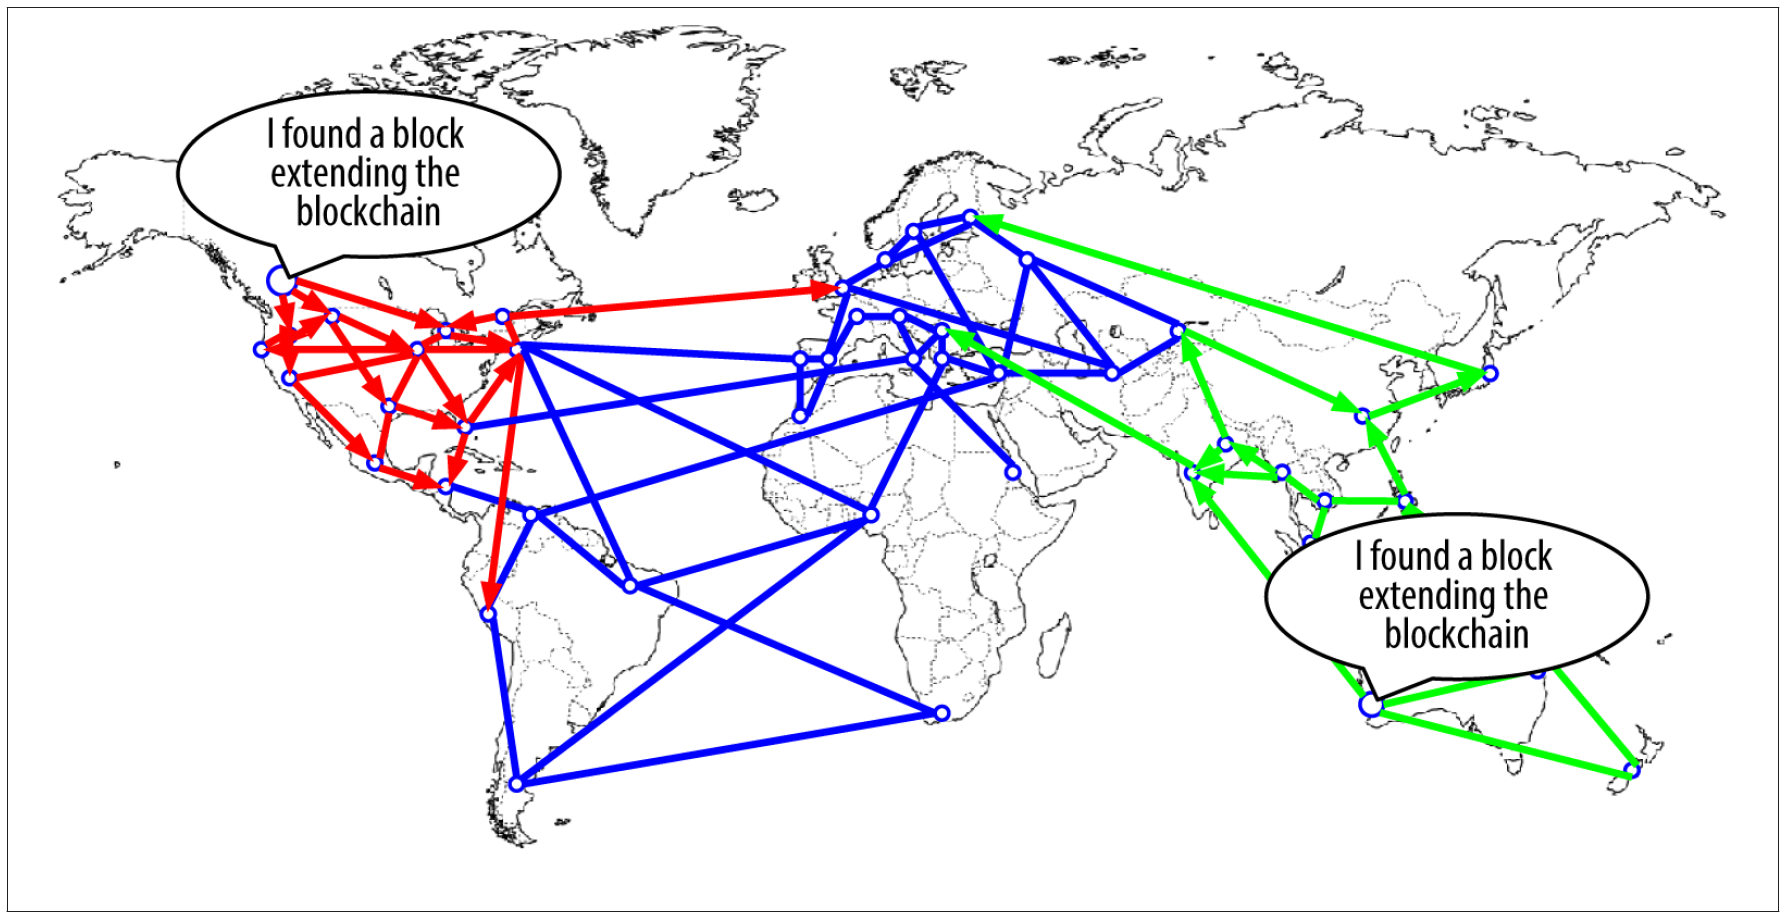
\includegraphics[width=0.85 \linewidth]{figure/fork2}
	\caption{\textit{Visualizzazione di un evento fork: due blocchi minati simultaneamente} \label{fig:fork2}}
\end{figure}

Per esempio, si assuma che un miner in Canada trova una soluzione proof of work per il blocco "rosso" che estende la blockchain come figlio del blocco "blu". Quasi simultaneamente, un altro miner in Australia trova un'altra soluzione per il blocco "verde" al fine di estendere la blockchain. Entrambi i blocchi sono validi, entrambi contengono una soluzione valida alla proof of work, e tutti e due sono figli del blocco "blu". Inoltre, entrambi contengono quasi le stesse transazioni, con solo alcune piccole differenze.

Appena i due blocchi vengono propagati, alcuni nodi ricevono il blocco "rosso" e altri il blocco "verde". Come si può vedere in \textit{figura \ref{fig:fork3}}, la rete si divide in due diverse prospettive della blockchain, un lato con all'estremità il blocco rosso e l'altro lato con il blocco verde.
\begin{figure}[htbp]
	\centering
	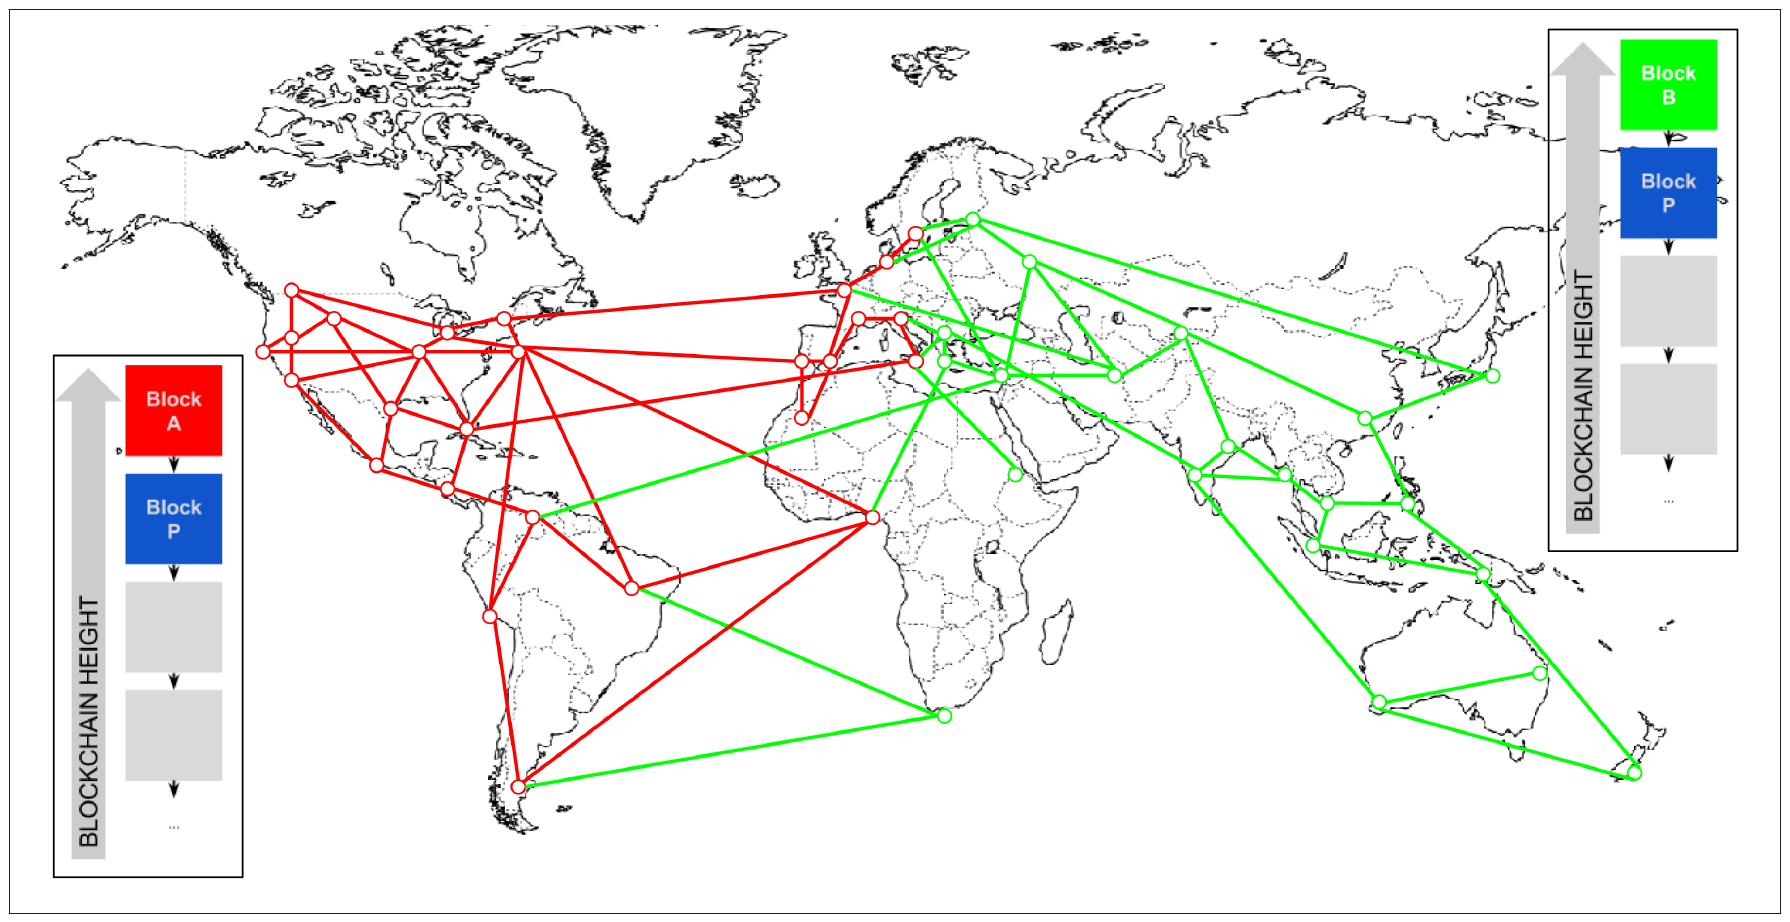
\includegraphics[width=0.85 \linewidth]{figure/fork3}
	\caption{\textit{Visualizzazione di un evento fork: due blocchi propagati, la rete biforca} \label{fig:fork3}}
\end{figure}

Da quel momento, i nodi della rete che sono più vicini al nodo del Canada, aggiungeranno anch'essi il blocco "rosso" per primo, e creeranno una nuova blockchain con il blocco "rosso" come ultimo blocco, ignorando il blocco "verde", che è arrivato un po' più tardi. Nello stesso momento, i nodi più vicini al nodo dell'Australia prenderà il blocco "verde" come vincitore e lo userà per estendere la sua versione della blockchain, aggiungendolo al blocco "blu", ignorando il blocco "rosso" che è arrivato un po' più tardi degli altri. Di conseguenza, ogni miner che vede aggiungere il blocco "rosso" in testa alla chain, immediatamente cercherà di creare altri blocchi che si aggiungeranno al blocco "rosso", ed andrà a risolvere la proof of work per tali blocchi candidati. Invece, i miners che accettano il blocco "verde" cominceranno ad estendere la porzione di chain che si andrà ad attaccare a tale blocco.

Le fork vengono quasi sempre risolte da un singolo blocco. Infatti, come parte del potere computazionale viene dedicato per aggiungere il blocco "rosso", un'altra parte della rete impiega le sue risorse per aggiungere il blocco "verde". Anche se il potere computazionale è quasi diviso in due parti, probabilmente un gruppo di miner troverà e propagherà la soluzione prima che lo faccia un altro gruppo di ulteriori miner. Per esempio, si supponga che i miner trovino un blocco "rosa" che estenda il blocco "verde", immediatamente lo propagherebbero all'intera rete (\textit{figura \ref{fig:fork4}}).
\begin{figure}[htbp]
	\centering
	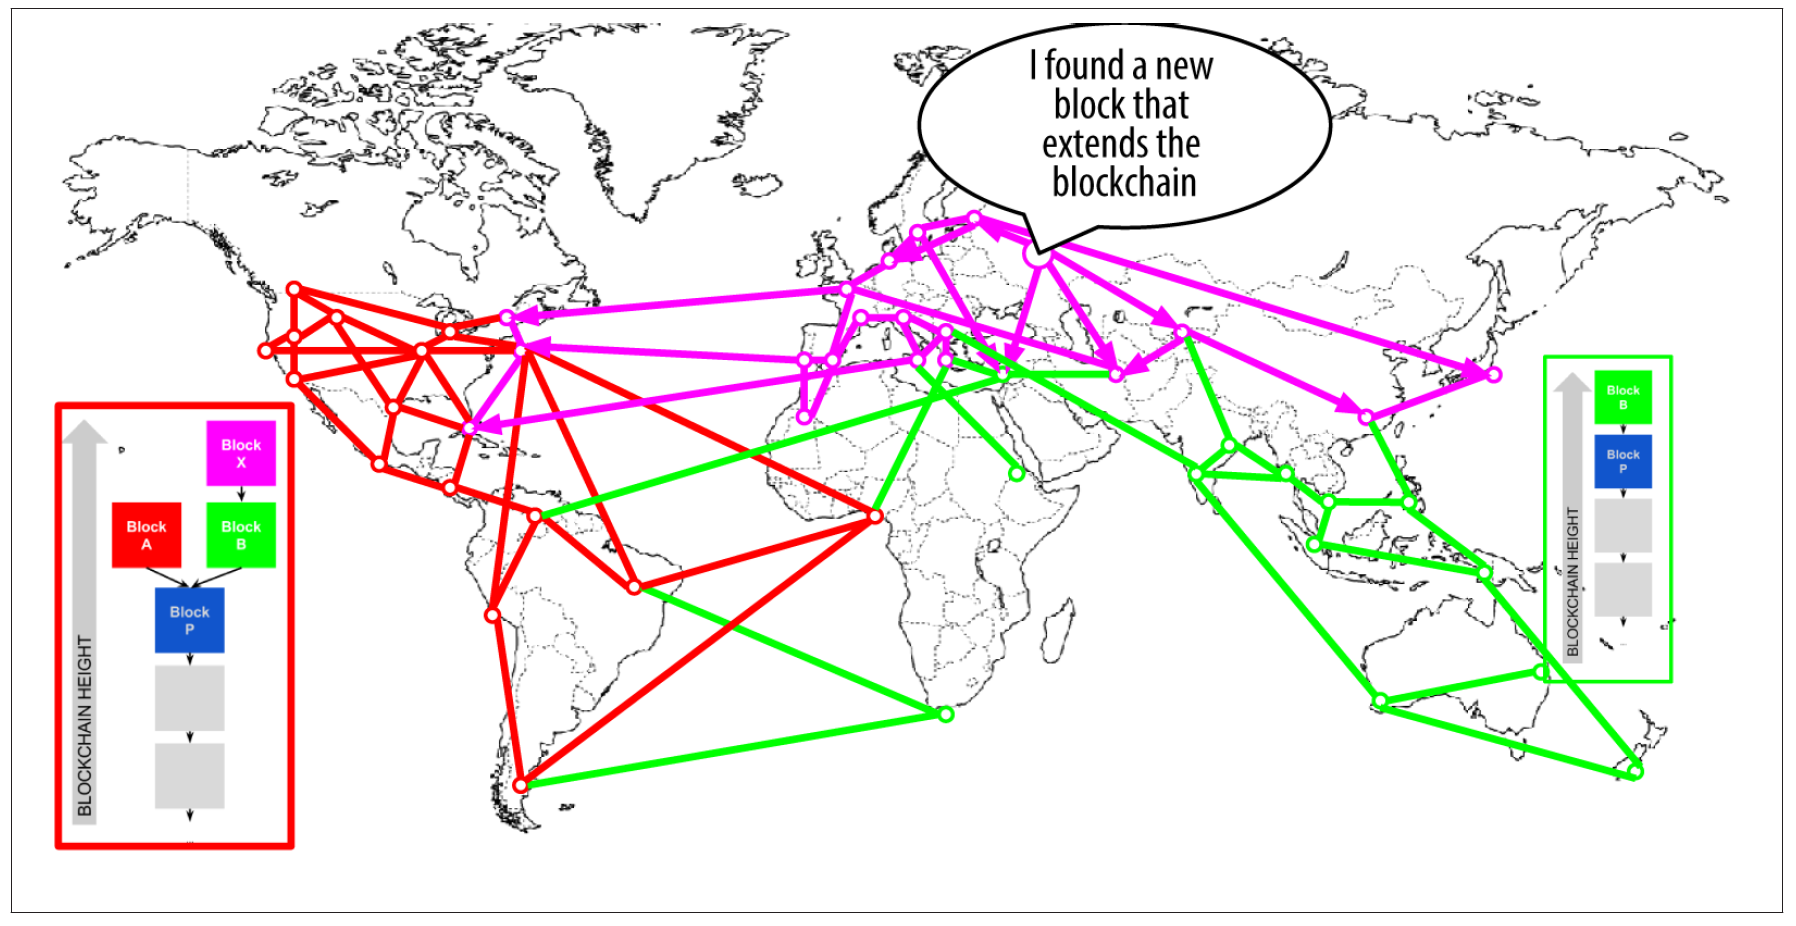
\includegraphics[width=0.85 \linewidth]{figure/fork4}
	\caption{\textit{Visualizzazione di un evento fork: un nuovo blocco estende un ramo della fork} \label{fig:fork4}}
\end{figure}

Tutti i nodi che hanno scelto il blocco "verde" come vincitore nel round precedente, estenderanno la catena di un ulteriore blocco. I nodi che hanno scelto il blocco "rosso" come vincitore, quindi, vedranno due chain: quella blu-verde-rosa e quella blu-rossa. La chain blu-verde-rosa è la più lunga, ovvero è più difficile trovare una prook of work per essa. Inoltre, in \textit{figura \ref{fig:fork5}} si possono vedere i nodi che hanno scelto come catena principale la chain blu-verde-rosa e come chain secondaria quella blu-rossa.

Questo processo è detto \textit{chain reconvergence}(letteralmente riconvergenza della catena), perchè tali nodi vengono forzati a cambiare il loro punto di vista della blockchain al fine di considerare la catena più lunga tra le due.\\ Ogni miner che lavora per estendere la chain blu-rossa non potrà più continuare poichè il blocco che stanno tentando di aggiungere al blocco rosso rimarrà "orfano", dato che il blocco rosso che dovrebbe fare da genitore non appartiene alla chain più lunga della blockchain. \\ Le transazioni che sono all'interno del blocco "rosso", vengono inserite di nuovo in coda per essere processate in un nuovo blocco, perchè, come si è già detto, il blocco a cui appartenevano non fa più parte della blockchain.
\begin{figure}[htbp]
	\centering
	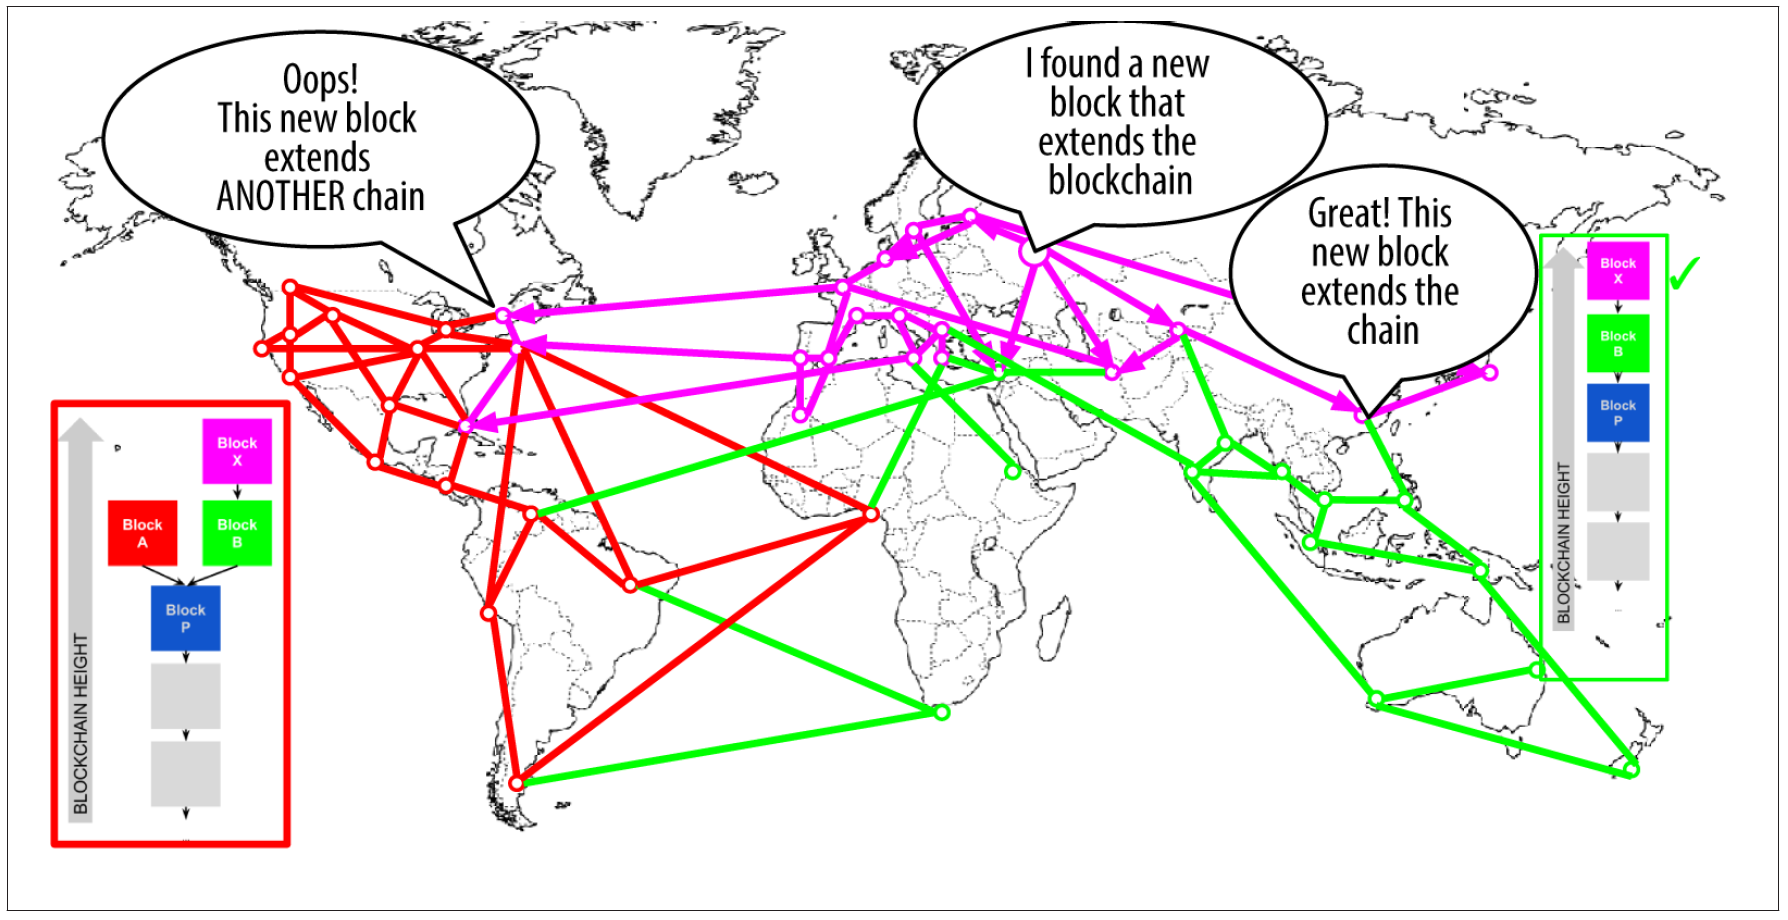
\includegraphics[width=0.85 \linewidth]{figure/fork5}
	\caption{\textit{Visualizzazione di un evento fork: la rete si riunisce in un'unica catena più lunga} \label{fig:fork5}}
\end{figure}
 
L'intera rete, quindi, riconverge la blockchain in una catena singola che fa capo ai blocchi blu-verde-rosa, con il blocco "rosa" come ultimo blocco all'estremità della catena. Tutti i miner immediatamente cominceranno a candidare nuovi blocchi che si andranno ad attaccare al blocco "rosa", al fine di estendere la catena blu-verde-rosa.

Teoricamente potrebbe essere possibile per una fork estendere due blocchi diversi, ma solamente se tali blocchi vengono creati quasi simultaneamente da miner che sono su "lati" diversi di una fork precedente. Tuttavia, la probabilità che ciò accada è molto bassa. Anche se ci fosse una fork ogni settimana, una fork a due blocchi è molto rara.

L'intervallo tra un blocco e il suo successivo è all'incirca di 10 minuti, proprio perché è stato progettato per essere un compromesso tra la velocità dei tempi di ricezione delle conferme e la probabilità di una fork. Un intervallo più ristretto da un lato potrebbe rendere le transazioni più veloci, dall'altro potrebbe causare fork più frequenti. Al contrario, un intervallo più ampio farebbe diminuire il numero delle fork ma renderebbe più lenti i pagamenti.\cite{antonopoulos2014mastering}

\subsection{Merkle Tree}

Ogni blocco della blockchain contiene un riepilogo di tutte le transazioni nel blocco, sotto forma di un \textbf{merkle tree}.

Un \textit{merkle tree}, altrimenti detto \textit{binary hash tree}, è una struttura dati usata per verificare e riepilogare efficientemente l'integrità dei dati. I merkle tree sono alberi binari composti da hash crittografici, dove ogni transazione è convertita in un hash, usando una funzione crittografica.

Il merkle tree è un albero perfettamente bilanciato, dove le foglie corrispondono agli hash delle singole transazioni. I nodi intermedi invece, sono calcolati applicando la funzione di hash alla concatenazione dei valori dei due figli (\textit{figura} \ref{fig:merkletree}).

\begin{figure}[htbp]
	\centering
	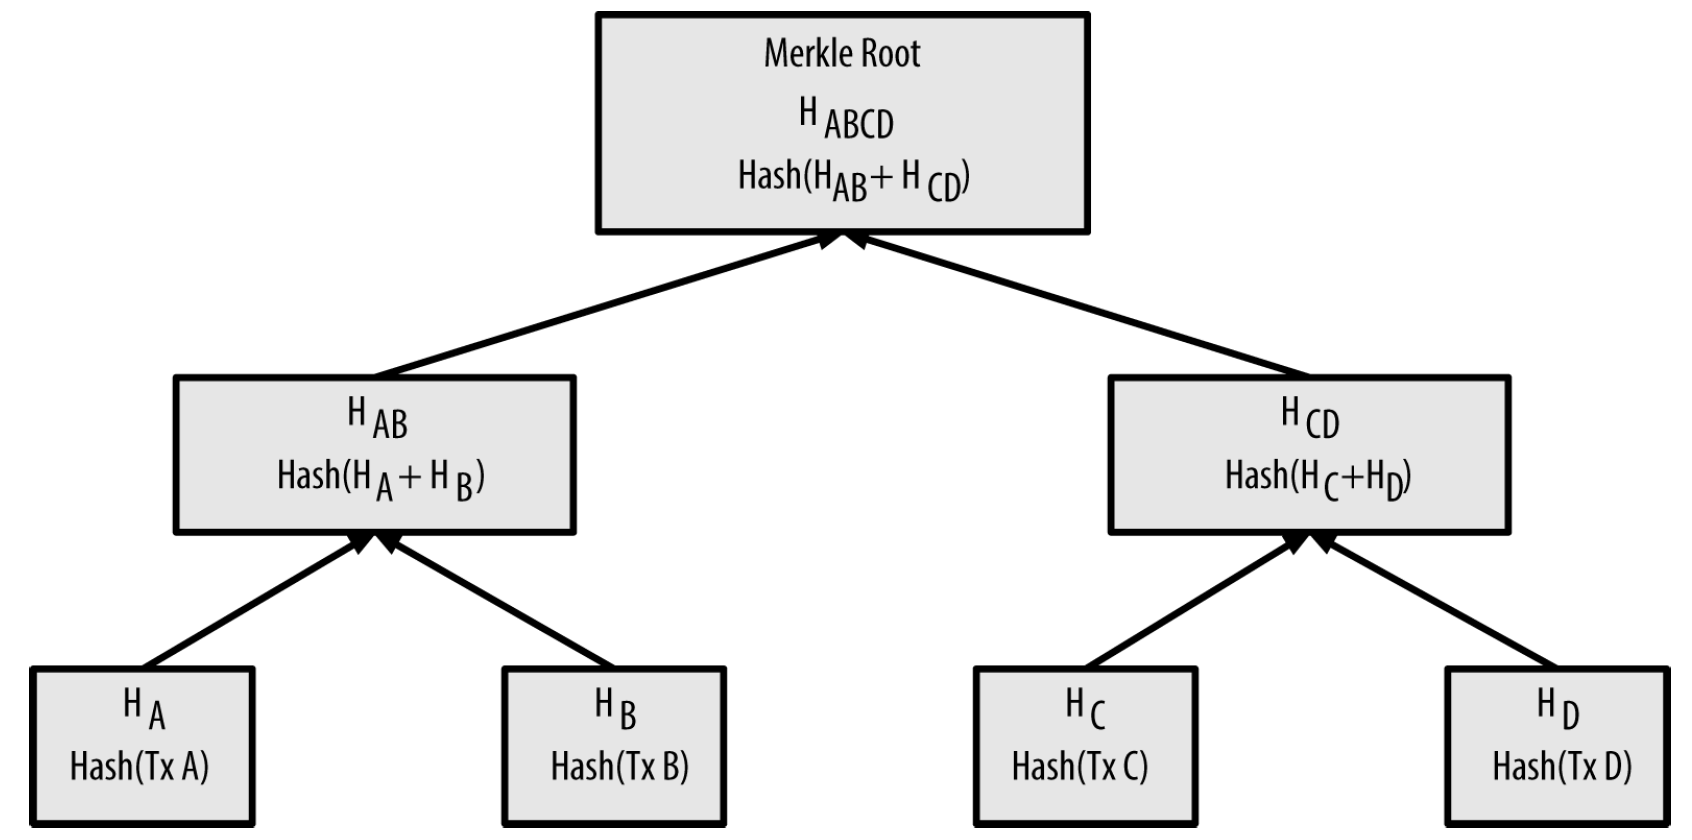
\includegraphics[width= 0.5 \linewidth]{figure/merkletree}
	\caption{\textit{Merkle tree} \label{fig:merkletree}}
\end{figure}

Nella figura si può notare una porzione di un albero merkle, che prende in considerazione quattro transazioni: Tx A, Tx B, Tx C e Tx D. L'albero in questione presenta delle caratteristiche diverse se il nodo è una foglia oppure è un nodo intermedio. Esso è costruito secondo l'approccio bottom-up, prima vengono calcolati gli hash delle foglie, poi man mano si arriva al calcolo della radice.

Le foglie dell'albero, vengono calcolate come hash delle quattro transazioni, quindi si avranno le quattro foglie rispettivamente: 
\begin{itemize}
	\item H$_A$ = Hash(Tx A)
	\item H$_B$ = Hash(Tx B)
	\item H$_C$ = Hash(Tx C)
	\item H$_D$ = Hash(Tx D)
\end{itemize}

Successivamente si calcola il valore dei genitori delle foglie. Infatti, ogni nodo tra di essi, viene calcolato facendo l'hash della concatenazione dei valori contenuti nelle foglie. Quindi per ogni nodo intermedio si avrà:
\begin{itemize}
	\item H$_{AB}$ = Hash(H$_A$+H$_B$) \footnote{In questo caso il simbolo + rappresenta la concatenazione}
	\item H$_{CD}$ = Hash(H$_C$+H$_D$)
\end{itemize}

Infine, la radice si ottiene facendo lo stesso procedimento dei nodi intermedi, ossia facendo la concatenazione dei valori contenuti nei nodi figli. In questo caso si otterrà:

H$_{ABCD}$ = Hash(H$_{AB}$+H$_{CD}$)

Nell'esempio appena visto, l'albero era un albero binario, dove il numero di transazioni risultava essere un numero pari. Se ci fosse un numero dispari di transazioni da considerare nel merkle tree, l'ultima transazione verrebbe duplicata ottenendo così un numero pari di transazioni. Si otterrà quindi un albero \textit{bilanciato}. In \textit{figura \ref{fig:merkletreedup}} viene mostrata la duplicazione della transazione Tx C, e di conseguenza della foglia a cui appartiene. \cite{antonopoulos2014mastering}

\begin{figure}[htbp]
	\centering
	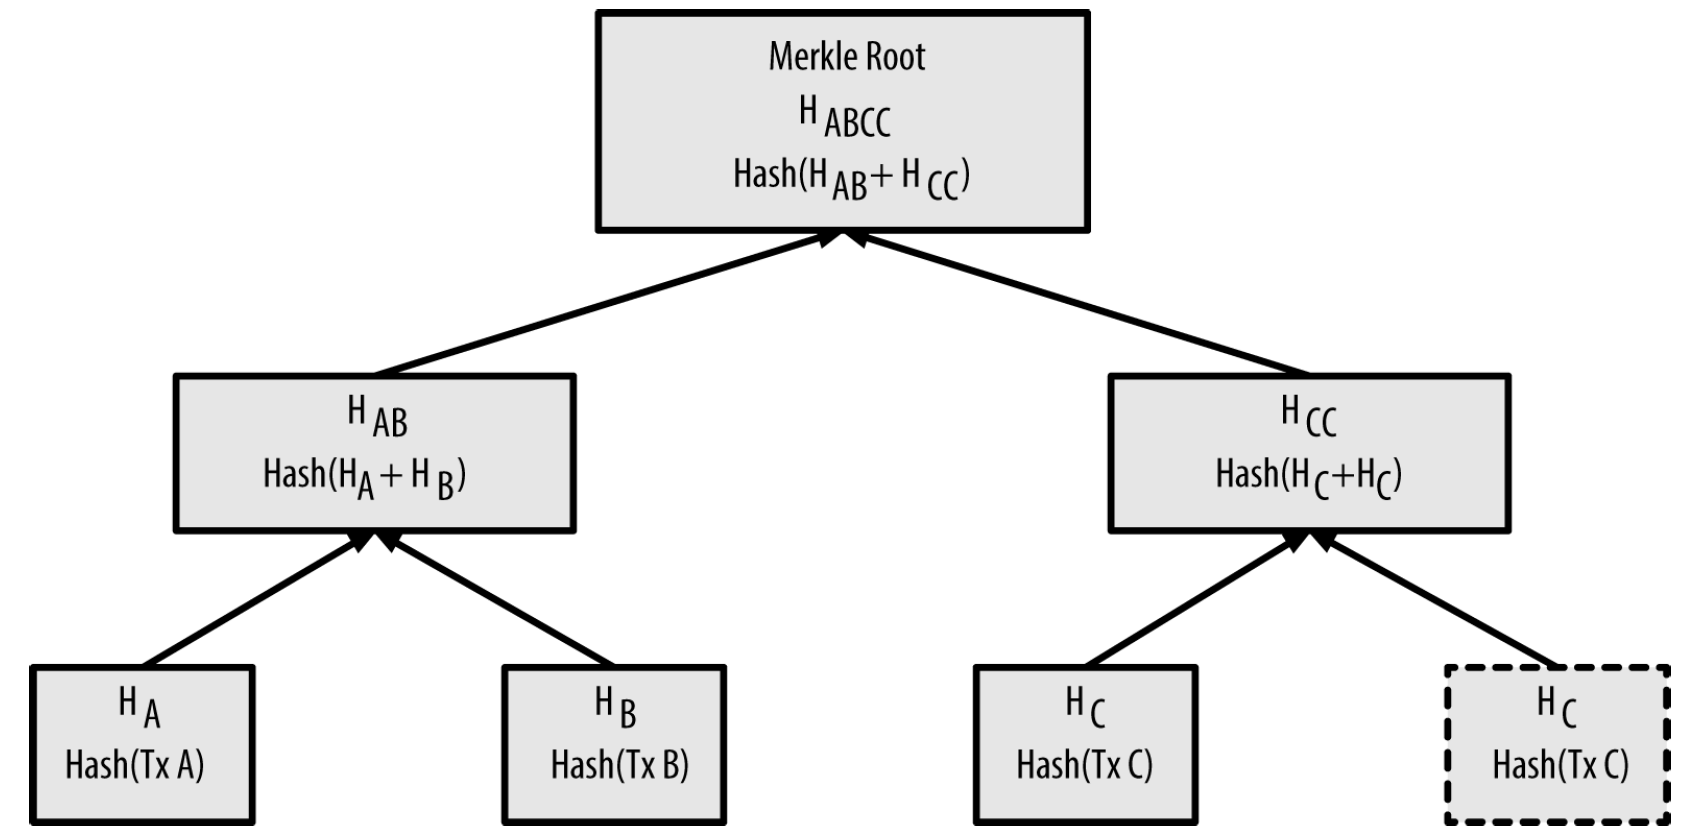
\includegraphics[width= 0.5 \linewidth]{figure/merkletreedup}
	\caption{\textit{Merkle tree con elemento duplicato} \label{fig:merkletreedup}}
\end{figure}

\section{Le Transazioni}

Come è stato detto in precedenza, una transazione è uno scambio di monete bitcoin tra due o più individui. Per esempio, se Alice vuole dare 1BTC a Bob, ha bisogno di effettuare una transazione inserendo come input l'importo da trasferire e l'indirizzo del wallet di Bob. \\ 

In parole semplici, la transazione dice alla rete che il proprietario di un certo numero di bitcoin, ha autorizzato il trasferimento di alcuni di tali bitcoin ad un altro individuo. Il nuovo proprietario dei bitcoin allora può spenderli creando una nuova transazione che autorizza il trasferimento degli stessi ad un altro destinatario. Tutto ciò genera una catena di proprietà di bitcoin.

Le transazioni sono come una riga in un registro di contabilità dove vengono salvati i trasferimenti. In poche parole, ogni transazione contiene uno i più input, cioè l'addebito, ed uno o più output, cioè il credito aggiunto ad un altro account bitcoin. Gli input e gli output, rispettivamente l'addebito e il credito, non necessariamente devono essere la stessa cifra. Infatti, gli output aggiungono all'account destinatario una cifra leggermente minore di quella inviata negli input, la cui differenza rappresenta le \textit{transaction fee}(ovvero le tasse di transazione), che vengono elargite al miner che ha minato il blocco nel quale andrà ad aggiungersi la transazione in corso. Nella \textit{figura \ref{fig:bookkeeping}} viene mostrata una transazione come sarebbe all'interno di un registro di contabilità.
\begin{figure}[htbp]
	\centering
	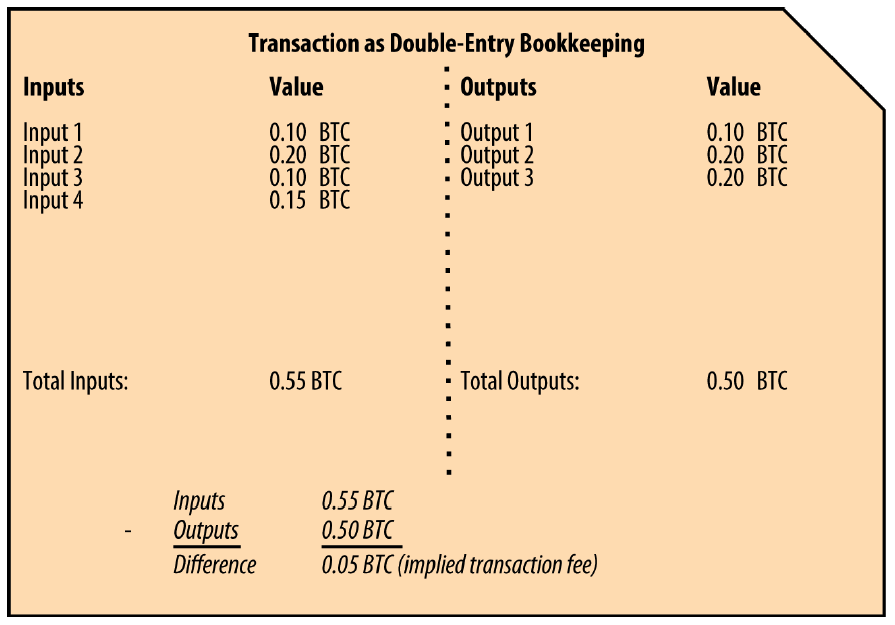
\includegraphics[width=0.7 \linewidth]{figure/bookkeeping}
	\caption{\textit{Una transazione come una riga del registro di contabilità} \label{fig:bookkeeping}}
\end{figure}

La transazione contiene anche la firma digitale del destinatario dell'importo dei bitcoin, in modo da fungere come prova di proprietà dal momento che nessun altro all'infuori del proprietario può validare la transazione e prendersi gli stessi bitcoin. In termini tecnici, "spendere" significa firmare una transazione che trasferisce il valore da una transazione effettuata in precedenza ad un nuovo proprietario identificato tramite il suo indirizzo bitcoin.

Le transazioni muovono ammontare di bitcoin da \textit{transazioni in input} a \textit{transazioni in output}. Un input è dove la moneta arriva da un output di una transazione effettuata in precedenza. Un output assegna un nuovo proprietario al valore scambiato, associandogli la chiave. La chiave di destinazione è chiamata \textit{encumbrance}(letteralmente "impedimento"). Esso impone l'esigenza di avere una firma che serve a riscattare i fondi in transazioni future. Gli output di una transazione possono essere utilizzati come input in una nuova transazione, creando così una catena di proprietà che rappresenta il valore che si muove da indirizzo a indirizzo (\textit{figura \ref{fig:chaintxs}}).
\begin{figure}[htbp]
	\centering
	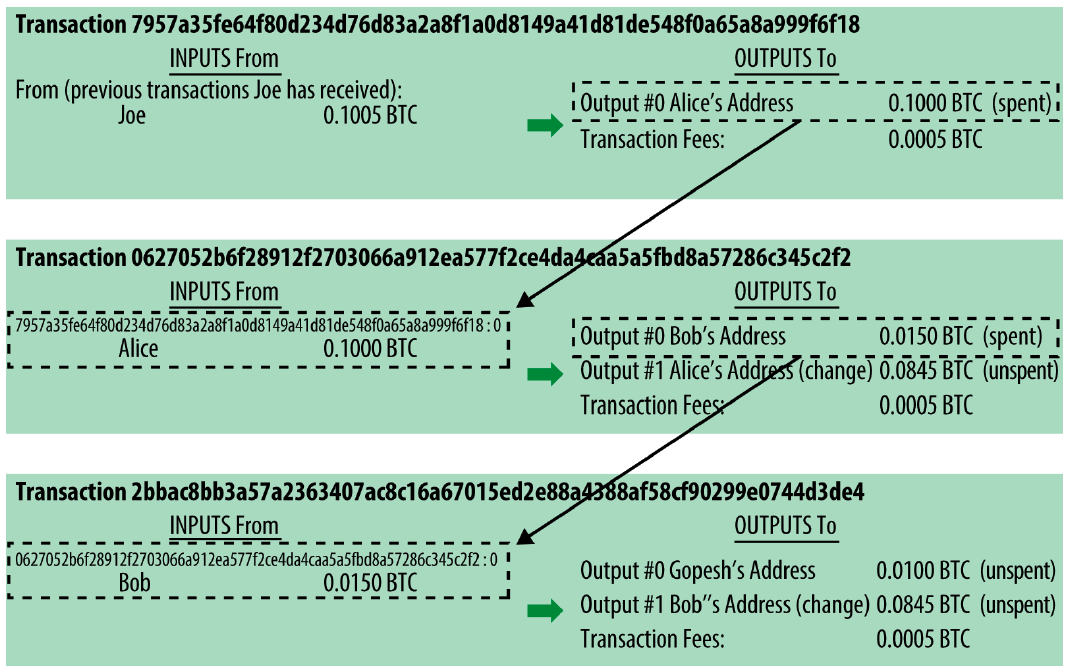
\includegraphics[width=0.7 \linewidth]{figure/chaintxs}
	\caption{\textit{Una catena di transazioni, dove l'output di una transazione viene utilizzato come input della transazione successiva} \label{fig:chaintxs}}
\end{figure}

Il pagamento di Alice al Bob's Cafe usa come input l'output di una precedente transazione. Infatti, prima di trasferire i suoi bitcoin a Bob, Alice li aveva ricevuti precedentemente da un suo amico Joe, che glieli aveva donati in cambio di una somma di denaro. Tale transazione ha un numero di bitcoin bloccati, che possono essere liberati solamente dalla chiave di Alice. La sua nuova transazione per pagare la tazza di caffè al bar di Bob fa riferimento come input alla transazione precedente e crea nuovi output grazie al pagamento. 

Le transazioni formano una catena, dove gli input dell'ultima transazione corrispondono ad output della transazione precedente. La chiave di Alice ha la funzione di firma che sblocca gli output della transazione precedente, proprio per provare alla rete bitcoin che Alice possiede tali monete. Lei attribuisce il pagamento all'indirizzo di Bob, in tal modo bloccando l'output che poi successivamente sarà sbloccato dalla chiave di Bob. Tutto ciò rappresenta il trasferimento di bitcoin tra Alice e Bob. La catena di transazioni che parte da Joe e arriva a Bob è illustrata in \textit{figura \ref{fig:chaintxs}}.\cite{antonopoulos2014mastering}

\subsection{Transaction Mining}

Quando viene fatta l'operazione di mining dei blocchi, vengono inserite le transazioni all'interno del nuovo blocco. In questa sezione viene mostrato il mining dal punto di vista della transazione.

In media ogni 10 minuti, i miner generano un nuovo blocco che contiene tutte le transazioni che sono state generate dopo l'ultimo blocco inserito. Le nuove transazioni scorrono all'interno della rete dai wallet degli utenti e da altre applicazioni. Appena le transazioni incontrano la rete di nodi bitcoin, vengono aggiunte ad una struttura dati temporanea presente in ogni nodo dove vengono conservate tutte le transazioni che non sono ancora state verificate. Appena i miner generano un nuovo blocco, aggiungono le transazioni non verificate da tale struttura dati, al nuovo blocco e tentano quindi di trovare la proof of work.

Prendendo in considerazione l'esempio precedente, la transazione di Alice quindi, viene prelevata dalla rete e inclusa all'interno della struttura dati temporanea. Essa viene aggiunta ad un blocco che accetta l'importo delle tasse pagate da Alice. All'incirca cinque minuti più tardi che la transazione è stata trasmessa dal wallet di Alice, un miner riesce a minare il blocco e pubblica il blocco contenente un certo numero di transazioni compresa quella di Alice. Il miner in questione pubblica il nuovo blocco sulla rete bitcoin, dove gli altri miner lo validano e possono continuare la corsa a trovare una nuova proof of work.

Pochi minuti più tardi, un nuovo blocco viene minato da un altro miner. Dal momento che un nuovo blocco viene aggiunto come figlio del precedente, il quale contiene la transazione di Alice, tale transazione aumenta la difficoltà di computazione della soluzione, rafforzando la fiducia su tali transazioni. Il blocco che contiene la transazione di Alice è considerato come una "conferma" aggiunta alle conferme della transazione in questione. Ogni blocco minato, quindi funge come conferma addizionale ad ogni transazione che contiene. 

Dal momento che i blocchi vengono impilati uno sopra l'altro, diventa esponenzialmente difficile invertire la transazione, in tal modo aumenta la fiducia della rete sulla Blockchain. 

Nella \textit{figura \ref{fig:aliceblock}} si può osservare il blocco \#277316 che contiene la transazione di Alice.
\begin{figure}[htbp]
	\centering
	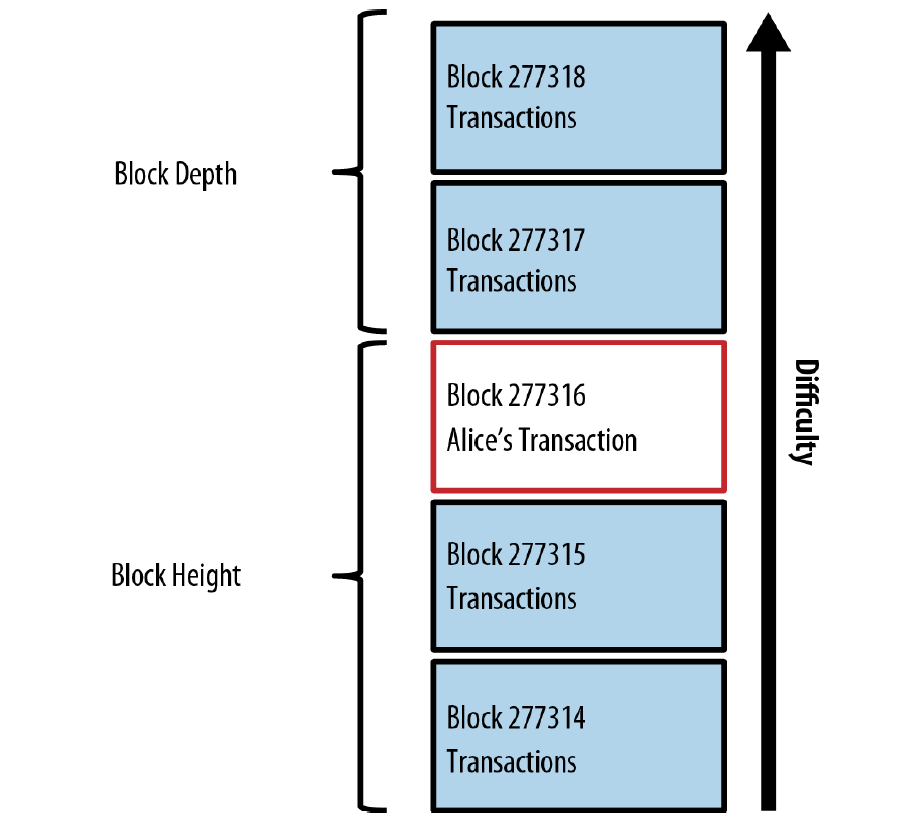
\includegraphics[width=0.5 \linewidth]{figure/aliceblock}
	\caption{\textit{La transazione di Alice inclusa nel blocco \#277316} \label{fig:aliceblock}}
\end{figure}

Ora che la transazione di Alice è inserita all'interno della blockchain, ogni client bitcoin può verificare se la transazione è valida e spendibile. Bob allora può spendere i bitcoin che ha ricevuto da Alice, prendendo tale output e usandolo come input per una nuova transazione. Appena Bob spende tali bitcoin, allunga la catena di transazioni. Si supponga che Bob paghi il suo web designer Gopesh, per un nuovo sito web. Quindi, la catena di transazioni viene mostrata in \textit{figura \ref{fig:abchaintxs}}.
\begin{figure}[htbp]
	\centering
	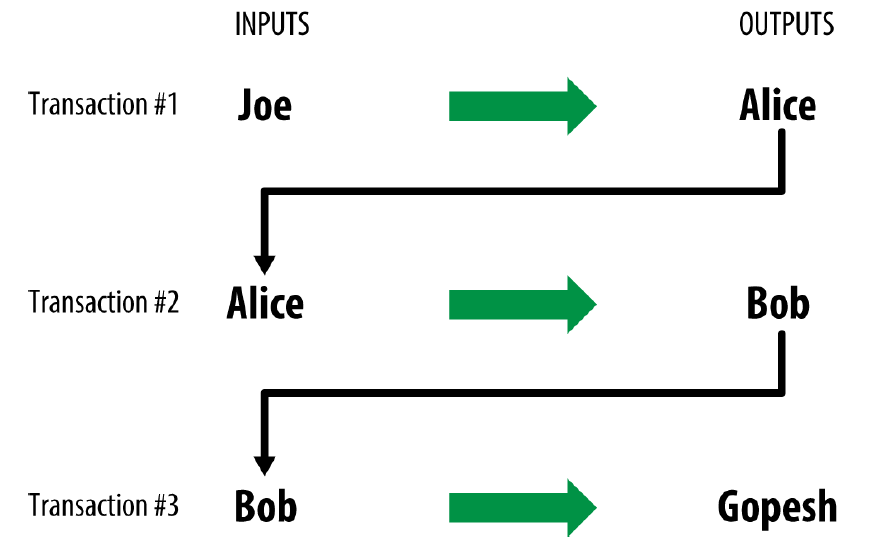
\includegraphics[width=0.5 \linewidth]{figure/abchaintxs}
	\caption{\textit{La transazione di Alice come parte di una catena di transazioni che va da Joe a Gopesh} \label{fig:abchaintxs}}
\end{figure}

\subsection{Forma Comune delle Transazioni}

La forma più comune di una transazione, è un semplice pagamento da un indirizzo ad un altro, in cui quasi sempre viene incluso il "resto" che ritorna al proprietario originale. Questo tipo di transazione ha un solo input e due output, di cui uno ha l'indirizzo pari all'indirizzo del mittente, tutto mostrato in \textit{figura \ref{fig:commontx}}.
\begin{figure}[htbp]
	\centering
	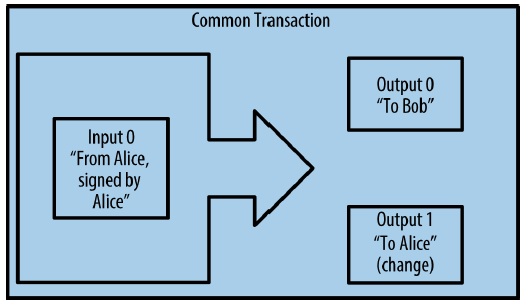
\includegraphics[width=0.5 \linewidth]{figure/commontx}
	\caption{\textit{Una comune transazione} \label{fig:commontx}}
\end{figure}

Un'altra forma comune è quella che aggrega molti input in un singolo output (\textit{figura \ref{fig:aggregatingtxs}}). Questo rappresenta il reale scambio di diverse somme di denaro, in un singolo importo. Le transazioni come queste molto spesso sono generate da wallet per pulire piccoli importi che sono stati ricevuti come resto di altri pagamenti.
\begin{figure}[htbp]
	\centering
	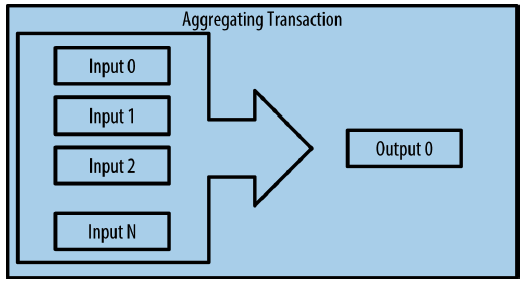
\includegraphics[width=0.5 \linewidth]{figure/aggregatingtxs}
	\caption{\textit{Aggregazione} \label{fig:aggregatingtxs}}
\end{figure}

Infine, un'altra forma può essere e quella che è il risultato di un'operazione in cui una singola transazione distribuisce il suo input su molti diversi output (\textit{figura \ref{fig:distributingtxs}}). Questo tipo di transazione viene utilizzata di solito da entità commerciali per distribuire i fondi, come quando un'azienda distribuisce il denaro come compenso ai propri dipendenti.	\cite{antonopoulos2014mastering}
\begin{figure}[htbp]
	\centering
	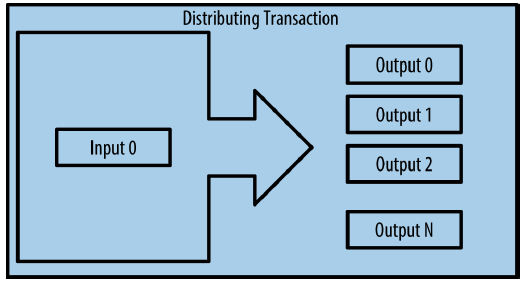
\includegraphics[width=0.5 \linewidth]{figure/distributingtxs}
	\caption{\textit{Distribuzione} \label{fig:distributingtxs}}
\end{figure}

\subsection{Struttura di una Transazione}
Una transazione è una struttura dati che racchiude un trasferimento di valori da una sorgente di fondi, chiamata \textit{input}, ad una destinazione, chiamata \textit{output}. Gli input e gli output non fanno riferimento ad account o ad identità. Al contrario, si potrebbe pensare ad esse come delle quantità di bitcoin -- gruppi di bitcoin -- che sono bloccati da una chiave crittografica. Solo il proprietario, possessore di tale chiave, può sbloccarli. Una transazione contiene dei campi di informazioni, come è mostrato nella \textit{tabella \ref{tab:txstructure}}.
\begin{table}[htbp]

	\begin{tabular}{r|c|c|c|}
		Size&Field &Description\\ \hline
		4 bytes&Version&Specifica le regole seguite dalla transazione\\
		1-9 byte (VarInt)&Input Counter&Numero degli input\\ 
		Variable&Inputs&Transazioni in input\\ 
		1-9 byte (VarInt)&Output Counter&Numero degli output\\
		Variable&Outputs&Transazioni in output\\
		4 bytes&Locktime&unix timestamp oppure il numero del blocco\\
		\hline
	\end{tabular}

	\caption{\textit{La struttura di una transazione}\label{tab:txstructure}}
\end{table}

Il campo \textbf{Locktime} (letteralmente "tempo di chiusura") definisce il primo istante in cui una transazione può essere aggiunta alla blockchain. Quando è uguale a zero, indica l'immediata esecuzione. 

Invece, se il locktime è maggiore di zero e minore di 500 milioni, è interpretato come l'altezza del blocco, ovvero significa che la transazione non è inclusa nella blockchain prima di specificare altezza del blocco. Se è maggiore di 500 milioni, è interpretato come un timestamp di tipo Unix Epoch (il numero di secondi dal primo Gennaio 1970) e la transazione non è inclusa nella blockchain prima di quell'istante specifico.


\subsection{Input e Output delle Transazioni}
L'elemento fondamentale di una transazione bitcoin è l'\textbf{unspent transaction output} (lettralmente "output di transazione non speso"), nella forma contratta \textbf{UTXO}.

Gli UTXO sono gruppi indivisibili di monete bitcoin che possono essere sbloccati solo dall'utente proprietario. Vengono registrati nella blockchain e riconosciuti come unità monetaria dall'intera rete.
La rete bitcoin ha tracciato tutti gli UTXO disponibili, e corrisponderebbero a milioni di bitcoin. Ogni volta che un utente riceve dei bitcoin, tale ammontare è registrato all'interno della blockchain sotto forma di UTXO. Quindi, un utente bitcoin potrebbe seminare migliaia di UTXO attraverso migliaia di transazioni e centinaia di blocchi. in effetti, non c'è nessun tipo di bilancio tra indirizzi bitcoin e output non spesi; ci sono solamente UTXO, che fanno capo a specifici proprietari. Il concetto di bilancio dell'utente in termini di output non spesi è un costrutto creato dall'applicazione che governa il wallet. Il wallet infatti, calcola il bilancio dell'utente scansionando la blockchain e aggregando tutti gli UTXO che appartengono a tale utente.

Un UTXO può avere un valore arbitrario che viene definito in termini di multipli di \textbraceleft{satoshi}. Come i dollari possono avere dei sottomultipli chiamati centesimi, i bitcoin possono essere divisi in satoshi. Ogni bitcoin corrispondono a $10^8$ satoshi.\cite{antonopoulos2014mastering}


\section{Grafo delle transazioni}

Come sottolineato nelle sezioni precedenti, le transazioni sono collegate tra loro sotto forma di chain. Ogni output di ogni transazione diventa un input per la transazione successiva. In questo modo le transazioni formano catene che si possono intersecare tra di loro.

Se consideriamo ogni transazione come un nodo e il collegamento input/output come gli archi, si ottiene un grafo, dove ogni componente connessa è una chain di transazioni connesse tra loro. Per ciò ogni catena di transazioni viene rappresentata come un gruppo di nodi-archi.

Si prenda in considerazione l'esempio visto in precedenza, della catena generata dalle transazioni di Joe, Alice, Bob e Gopesh (\textit{figura} \ref{fig:abchaintxs} di pagina \pageref{fig:abchaintxs}). Alice riceve i bitcoin da Joe, poi li usa per pagare il caffè al bar di Bob, infine quest'ultimo utilizza una parte di tali bitcoin per pagare il suo web designer Gopesh.

In \textit{figura \ref{fig:threenodes}} si può vedere come una catena di transazioni viene convertita in un grafo. In questo caso il grafo è un cammino, ovvero una sequenza di nodi collegati da archi, dove ogni nodo ha un solo predecessore ed un solo successore.

\begin{figure}[htbp]
	\centering
	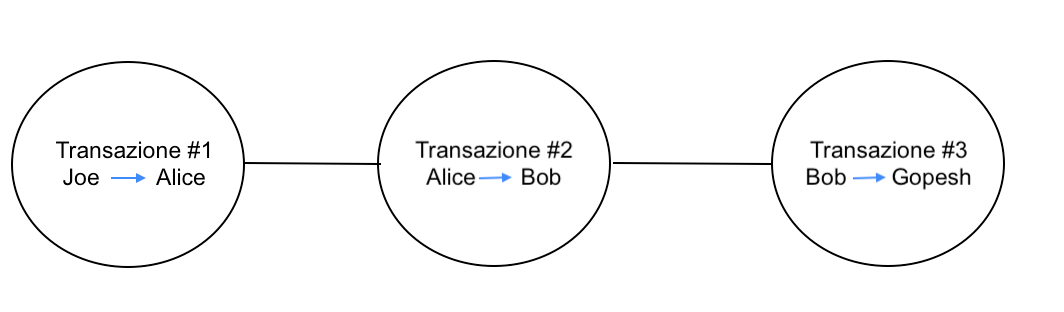
\includegraphics[width=\linewidth]{figure/threenodes}
	\caption{\textit{Grafo delle transazioni} \label{fig:threenodes}}
\end{figure}


\section{Caratteristiche del grafo}

testo testo 
testo